\paragraph{When will recruitment and data collection commence?}


Recruitment of participants and data collection will commence on August 15th, 2018. Data collection will begin on September 3rd, 2018.
\paragraph{When will data collection be completed?}


Data collection will be completed by September 15th, 2018.
\paragraph{7.	Brief description in lay terms of the aim of the project, and outline of the research questions that will be answered (approx. 200 words):}


In my system users are able.. [brief description of the system]

The aim of the system is to analyze \gls{wa} of an architectural \gls{vr} application in a collaborative setting with and without additional auditory cues. \newline

Research questions: Can \gls{wa} in an architectural \gls{vr} application be improved by providing additional spatialized auditory cues from the environment? \newline

The system simulates the presence of 2 users in the same collaborative virtual environment in an architectural context: one user is the participant and the other is simulated by scipting the movements of a \gls{vb}. The translations of \gls{vb}s can be followed by an auditory cue in a shape of recording of a sound of concrete moving on concrete (\textbf{\textit{github link?}}). The participant observes the environement through an \gls{hmd}, and manipulates it with the help of controllers. User can get additional cues about the environment from the radar view - a minimap showing surrondings.  \newline

As \gls{wa} is a secondary activity by nature, the participants will have a main task, where they have to fill in a 3D shape. This task tries to mimic the 3D sketching capabilitities of the \gls{cdp} system. To analyze the \gls{wa}, a \gls{vb} in the scene will translated by a script at along certain paths at certain moments in time. The participants will be asked to indicate that they have noticed this translation, pinpoint the perceived position of the \gls{vb}, and its direction of translation (Fig. \ref{fig:query_direction}). 

\begin{figure}%
	\centering
	\subfloat[]{{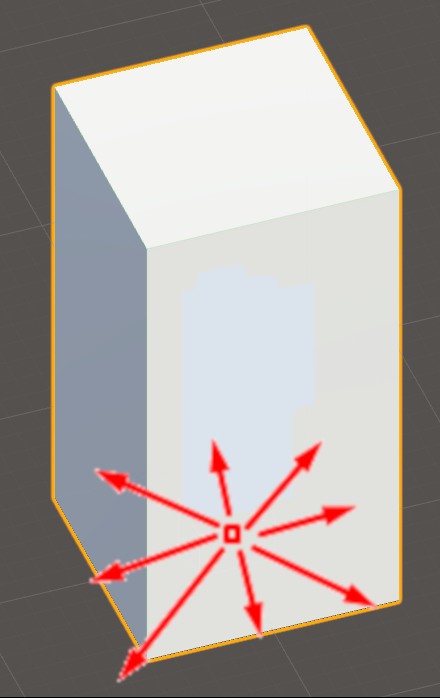
\includegraphics[width=3cm]{figures/final_experiment/directionSelection1.png} }}%
	\qquad	
	\subfloat[]{{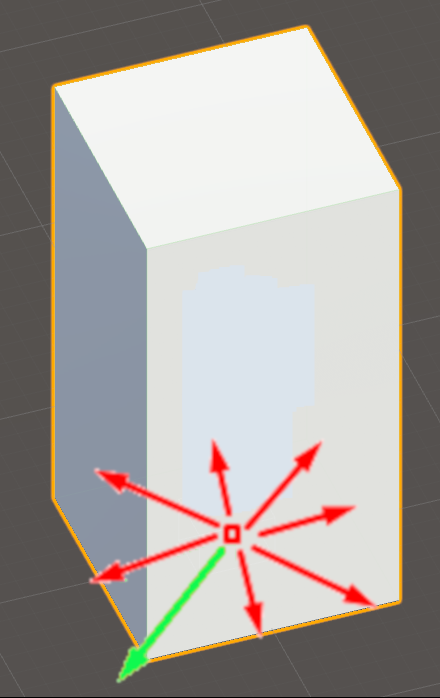
\includegraphics[width=3cm]{figures/final_experiment/directionSelection3.png} }}%	
	\qquad
	\subfloat[]{{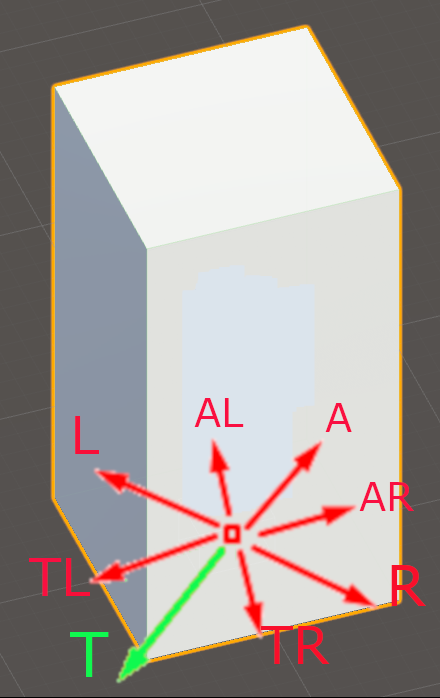
\includegraphics[width=3cm]{figures/final_experiment/directionSelection3Named.png} }}%
	\caption{Quering for direction of translation}%
	\label{fig:query_direction}%
\end{figure}



\paragraph{8.	Brief description of the method.} Include a description of who the participants are, how the participants will be recruited, and what they will be asked to do and how the data will be used and stored (Note: if this research involves patient data or health information obtained from the Ministry of Health, DHBs etc please refer to the UOHEC(H) Minimal Risk Health Research  - Audit and Audit related studies ):-

\paragraph{Experimental Design}

The independent variables are 1) auditory cues from moving \gls{vb}s and 2) a visual Radar view (minimap) of the surrounding environment. Auditory cues have 2 levels: turned on and muted. The radar has 2 levels also: shown and hidden.
The dependent variables will be \gls{wa}-related measurements: speed of the reaction when "catching" a \gls{vb} (\gls{sa} Levels 1,2: Perception and Comprehension), and the correctness in specifying it's translation direction (i.e. away from you, towards you, parallel to the left, etc.; \gls{sa} Level 3: Projection).

I am using a within-subjects experimental design, which consists of 3 groups:
\begin{enumerate}
	\item Auditory cues turned on, Radar hidden.
	\item Auditory cues turned on, Radar shown.
	\item Auditory cues.
\end{enumerate}
All participants will be tested in each group, but the order in which they are presented will be randomized to satisfy parametric assumption of unbiased results by eliminate the learning effect. The experiment will take approximately 30 minutes in total.

\paragraph{Participants}
Participants will be recruited from the \gls{tum}. This can include undergraduate students, postgraduate students, support staff, academic staff and lecturers/professors. All participants wouldn't have experienced the system before to insure independent samples.

\paragraph{Recruitment}
(Isn't my target group - architects?) The recruitment will be done via promoting the project at the chair for Architectural Informatics from the faculty of Architecture at the \gls{tum}, as well as by inviting friends to take part. 

\paragraph{Reward}
Participants will be thanked and offered a chocolate bar at the conclusion of their session.

\paragraph{Estimated Number of participants}
I estimate requiring 12 or more participants, with the number of participants being a multiple of 6. This is based on the previous study by \cite{gutwin_chalk_2011} and the number of possible permutations of the 3 groups in my experiment design ($P_{3}=6$).


\paragraph{Participant Inclusion and exclusion criteria:}
\begin{enumerate}
	\item Participants must have normal, or corrected to normal vision
	\item Participants must speak English in order to answer questionnaires 
	\item Participants must have no upper limb impairments to either limb (left or right arm)
	\item Participants must have no impairment to either hand which affects their use of the hand/fingers or has pain in using either hand/fingers.
	\item Participants must be comfortable wearing and using a head-mounted display device and stereo headphones. 
\end{enumerate}

\paragraph{Questionnaires and Measures} \mbox{} \newline \newline
\textit{Self-report Questionnaires} \newline
\begin{enumerate}
	\item Simulator Sickness questionnaire (Virtual Reality sickness or Cybersickness?)
	\item SBSOD, short for Santa Barbara Sense of Direction (Hegarty et al. 2002), is a self-report measure for measuring people’s judgments about environmental spatial abilities \cite{jr_3d_2017}  \newline
\end{enumerate}

\textit{Performance} \newline
The system will collect the following data:
\begin{enumerate}
	\item The fact of "catching" the \gls{vb}.
	\item The time it took for participant to catch the \gls{vb}, counting from the initiation of it's tranlation.
	\item \gls{vb} translation direction guess.
\end{enumerate}


\paragraph{Procedure}

Data will be collected from the participants from the questionnaires as well information collected via the system. The experiment will take approximately 30 minutes. Before the experiment begins, all participants are provided with information sheets and consent forms, which explains the experiment in detail. If they agreed and signed the consent forms, they proceed to the experiment. The participants will begin by filling out the Demographic Survey. They will then complete the Hand Visualization Realism Questionnaire which has participants evaluate the 4 hand visualizations in terms of realism. This is done to replicate the previously described study and allow for our findings to factor in realism of the hand visualizations.
Before the session, the participants will be explained the system set up and be demonstrated how it works. Instructions will be given to ensure the system is operated with a flat hand or index finger on the desk/table instead of having the hand in mid-air. Participants will be randomly assigned one of the four hand visualizations. Participants will be asked to play a “warm up” game with their assigned hand visualization. The “warm up” game has a similar tile board to TheraMem, however, has a different task. The task is to use the hand visualization to move the visualized hand/finger to a colour identified tile (repeat for 10 tiles). The purpose of the warm up task is to get the participant comfortable with the game interaction without having them practice the actual TheraMem game. The participant will play the warm up game twice (both mirrored and non-mirrored).
Once participants understand how to play the game, the procedure for rounds of the game will be explained. The order of the mirroring conditions will be randomly assigned. The participant will then play a round of TheraMem with their assigned hand visualization and given starting mirroring condition. Each round of the game will take approximately 2-4 minutes. After each round of the game, they will be asked to answer 16 Session Self-Report Sheet questions. The previous participant answers will be displayed to the participant so that they will be able how they answered questions from previous round to give a relative (differential) judgement. They will play a total of two rounds of TheraMem in the experiment (one for each mirroring condition).
At the conclusion of the experiment, participants will be informed of the actual difference between the conditions and will be asked not to reveal this to peers for the immediate future. They will be asked if they would like to receive the results of the study and asked about their interest in participating in future studies. All participants will be thanked and given a chocolate bar. 

\paragraph{Data Storage}

The results of the project may be published and will be available in the Technical University of Munich Library (Munich, Germany) but every attempt will be made to preserve anonymity.

\paragraph{Disclose and discuss any potential problems and how they will be managed}
Generally, I do not anticipate any problems arising out of this experiment for participants. However, there might be some fears about the confidentiality and anonymity of participants. Regarding this, participants will be informed that their participation is voluntary and that all their details will be kept confidential and anonymous. No sensitive information will be collected. Each participant will be provided with an information sheet and a consent form to read explaining this before starting the experiment. 
Experiencing virtual reality and wearing a head-mounted display can cause unintended temporary side effects. Rare temporary side effects of experiencing virtual reality can include motion sickness, eye discomfort and fatigue. These side effects are temporary and there are no reported cases of them being permanent. We don’t foresee these side effects occurring; however, we will screen participants if they are predisposed to motion sickness or have had any negative experiences in virtual reality before. If they are predisposed to motion sickness or have had negative experiences using virtual reality in the past, they will be warned about the possibility of experiencing those again. I have taken steps to mitigate potential motion sickness by using modern hardware (HTC Vive HMD), which have low latency and high frame update rate. However, if these rare side effects do occur, the participant will stop the experiment for the moment and take a break. They will be informed that they can stop the experiment if they wish or they can continue if the side effect has alleviated. 
It is possible that the outcome of this project will be used by other reports, publications or conferences. In this situation, no individuals will be identified. 
